\begin{figure}[H]
\centering
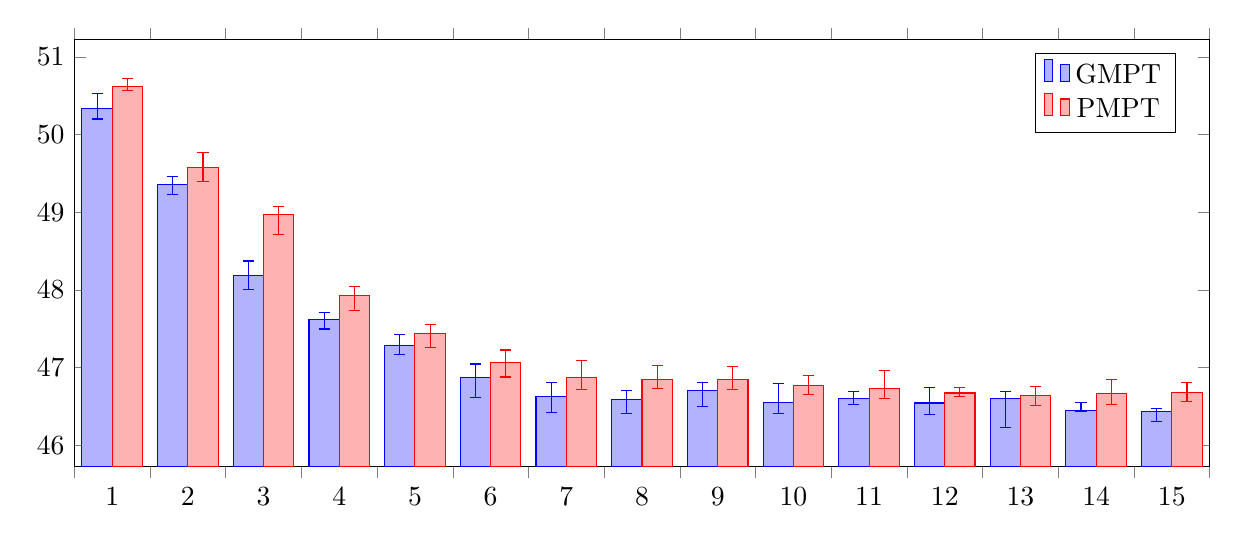
\begin{tikzpicture}
\begin{axis}[
legend pos=north east,
enlargelimits={abs=0.5},
ybar=0pt,
bar width=0.4,
width=16cm,
height=7cm,
xtick={0.5,1.5,...,15.5},
xticklabels={1,...,15},
x tick label as interval
]

\addplot+[error bars/.cd,
y dir=both,y explicit]
coordinates {
    (1,50.33937656) += (0,0.190813545) -= (0,0.137915825)
    (2,49.35669222) += (0,0.104331085) -= (0,0.130885005)
    (3,48.19097365) += (0,0.182186825) -= (0,0.185316615)
    (4,47.62424634) += (0,0.08795757) -= (0,0.12597638)
    (5,47.29060274) += (0,0.141786355) -= (0,0.118604915)
    (6,46.87572704) += (0,0.171886835) -= (0,0.265116815)
    (7,46.62973911) += (0,0.17877497) -= (0,0.20927576)
    (8,46.5920789) += (0,0.114632095) -= (0,0.183715455)
    (9,46.70301373) += (0,0.10315522) -= (0,0.20065271)
    (10,46.54843634) += (0,0.25140397) -= (0,0.14171314)
    (11,46.59903249) += (0,0.09624692) -= (0,0.07110101)
    (12,46.54537319) += (0,0.202520475) -= (0,0.148703605)
    (13,46.59768422) += (0,0.09747961) -= (0,0.36892214)
    (14,46.44280198) += (0,0.112942395) -= (0,0.012193785)
    (15,46.4338047) += (0,0.038619905) -= (0,0.123998935)};
\addplot+[error bars/.cd,
y dir=both,y explicit]
coordinates {
    (1,50.61976356) += (0,0.101523985) -= (0,0.053735465)
    (2,49.57587518) += (0,0.193009565) -= (0,0.181597855)
    (3,48.96792975) += (0,0.109636005) -= (0,0.249692145)
    (4,47.92520965) += (0,0.12491812) -= (0,0.18365727)
    (5,47.43763138) += (0,0.112263245) -= (0,0.173705345)
    (6,47.06281095) += (0,0.165015985) -= (0,0.183683195)
    (7,46.87233309) += (0,0.21922551) -= (0,0.14813599)
    (8,46.84258858) += (0,0.19058075) -= (0,0.10687422)
    (9,46.84206717) += (0,0.171504615) -= (0,0.119597965)
    (10,46.7723845) += (0,0.121608455) -= (0,0.122962645)
    (11,46.72814892) += (0,0.23062294) -= (0,0.12541048)
    (12,46.67324933) += (0,0.06953023) -= (0,0.04985557)
    (13,46.64070392) += (0,0.118115005) -= (0,0.131196595)
    (14,46.66670041) += (0,0.18079879) -= (0,0.13679915)
    (15,46.68468602) += (0,0.12580603) -= (0,0.11506425)};
\legend{GMPT,PMPT}
\end{axis}
\end{tikzpicture}
\caption[Comparison Multi-Task Raspberry]{Comparison\footnotemark of the temperature measurements for GMPT and PMPT}
\label{fig:i_eva_mabar_pi}
\end{figure}
\footnotetext{The bar values correspond to the median and the error bars correspond to the lower and upper inner fences displayed in the boxplots in \autoref{fig:i_eva_mabar_pi}}